\documentclass[12pt,twoside]{mitthesis-exec}

%%%%%%%%%%%%%%%%%%%%%%%%%%%%%%%%%%%%%%%%%%%%%%%%%%%%%%%%%%%%%%%%%%%%%%%%%%%%%%%%
% PREAMBLE

\usepackage[bitstream-charter]{mathdesign} % Use BT Charter font
\usepackage[T1]{fontenc}                   % Use T1 encoding instead of OT1
\usepackage[utf8]{inputenc}                % Use UTF8 input encoding
\usepackage{microtype}                     % Improve typography
\usepackage{amsmath}                       % AMS Math extensions
\usepackage{booktabs}                      % Improve table spacing
\usepackage{graphicx}                      % Extended graphics capabilities
\usepackage{tocbibind}                     % Include listings in TOC
\usepackage[printonlyused]{acronym} % withpage: for showing page of use
\usepackage{listings}                      % Source code listings
\usepackage{caption}
\usepackage{subcaption}
\usepackage[rgb,table]{xcolor}
\usepackage{url}
\usepackage{soul}
\usepackage{array}
\usepackage{pdfpages}
\usepackage{mathtools}
\usepackage{setspace}
\usepackage{pbox}
\usepackage{tikz}
\usetikzlibrary{calc,shapes,decorations.pathreplacing,positioning}
\usepackage{pgfplots}
\usepackage{siunitx}
\usepackage{multirow}
\usepackage{breqn}

% Specialties for tables
\usepackage{array}
\newcolumntype{L}[1]{>{\raggedright\let\newline\\\arraybackslash\hspace{0pt}}m{#1}}
\newcolumntype{C}[1]{>{\centering\let\newline\\\arraybackslash\hspace{0pt}}m{#1}}
\newcolumntype{R}[1]{>{\raggedleft\let\newline\\\arraybackslash\hspace{0pt}}m{#1}}

\usepackage[breaklinks=true]{hyperref}
\hypersetup{colorlinks=true, linkcolor=black, citecolor=black, urlcolor=black,
  pdftitle={Full Core 3D Neutron Transport Simulation Using the Method of Characteristics with Linear Sources},
  pdfauthor={Geoffrey Alexander Gunow}
}
\pagestyle{plain}

%\usepackage{floatrow}
%\floatsetup[table]{style=plaintop}
%\floatsetup[widefigure]{margins=hangleft}

% Highlights and emphasis boxes from Bryans thesis
\usepackage[framemethod=tikz]{mdframed}
\definecolor{mitred}{rgb}{0.698,0.0314,0.216}
\definecolor{mitgray}{rgb}{0.690,0.694,0.710}
\definecolor{canyellow}{rgb}{0.933, 0.965, 0.424}
\newmdenv[nobreak=false, skipabove=2ex, skipbelow=2ex, innerlinewidth=3pt, innerlinecolor=black, backgroundcolor=mitgray!75, roundcorner=10pt, frametitlerule=true, frametitlerulewidth=2.5pt, frametitlefont=\color{white}\Large\bfseries, frametitlealignment=\centering, frametitlebackgroundcolor=mitred, frametitleaboveskip=2ex, frametitlebelowskip=2ex, innertopmargin=3ex, innerbottommargin=2ex]{highlightsbox}
\newmdenv[nobreak=false, skipabove=2ex, skipbelow=2ex, innerlinewidth=2pt, innerlinecolor=black, backgroundcolor=white, roundcorner=10pt]{emphbox}

% Appendix
\usepackage[toc,page]{appendix}

% Don't reset footnote counter between chapters
\usepackage{chngcntr}
\counterwithout{footnote}{chapter}

% Algorithm constructs
\usepackage[chapter]{algorithm} % Provides algorithm environment
\usepackage{algorithmicx}       % Provides algorithmic block
\usepackage{algpseudocode}      % Option of algorithmicx package
\renewcommand{\thealgorithm}{\thechapter-\arabic{algorithm}}
\newcommand\Algphase[1]{%
\vspace*{-.7\baselineskip}\Statex\hspace*{\dimexpr-\algorithmicindent-2pt\relax}\rule{\columnwidth}{0.4pt}%
\Statex\hspace*{-\algorithmicindent}{#1}%
\vspace*{-.7\baselineskip}\Statex\hspace*{\dimexpr-\algorithmicindent-2pt\relax}\rule{\columnwidth}{0.4pt}%
}
\newcommand{\algrule}[1][.4pt]{\par\vskip.5\baselineskip\hrule height #1\par\vskip.5\baselineskip}

% Configure captions
\captionsetup{labelfont=bf, labelsep=colon}
\captionsetup[algorithm]{labelfont=bf, labelsep=colon}

% Use Latin Modern for typewriter fonts
\renewcommand{\ttdefault}{lmtt}

% Add \unit macro
\newcommand{\unit}[1]{\ensuremath{\, \mathrm{#1}}}

\definecolor{gray}{rgb}{0.4,0.4,0.4}
\definecolor{darkblue}{rgb}{0.0,0.0,0.6}
\definecolor{cyan}{rgb}{0.0,0.6,0.6}
\lstset{
  basicstyle=\footnotesize\ttfamily,
  columns=fullflexible,
  showstringspaces=false,
  commentstyle=\color{gray}\upshape,
  frame=single,
  xleftmargin=0.55in
}

\lstdefinelanguage{XML}
{
  morestring=[b]",
  morestring=[s]{>}{<},
  morecomment=[s]{<?}{?>},
  morecomment=[s]{<!--}{-->},
  stringstyle=\color{black},
  identifierstyle=\color{darkblue},
  keywordstyle=\color{cyan},
  morekeywords={}
}

\setcounter{secnumdepth}{4}
\setcounter{tocdepth}{3}

\renewcommand{\contentsname}{Table of Contents}
\renewcommand{\bibname}{References}

\makeatletter \renewcommand\thealgorithm{\arabic{algorithm}} \@addtoreset{algorithm}{chapter} \makeatother

\begin{document}

%%%%%%%%%%%%%%%%%%%%%%%%%%%%%%%%%%%%%%%%%%%%%%%%%%%%%%%%%%%%%%%%%%%%%%%%%%%%%%%%
% TITLE PAGE

% -*-latex-*-
% 
% For questions, comments, concerns or complaints:
% thesis@mit.edu
% 
%
% $Log: cover.tex,v $
% Revision 1.8  2008/05/13 15:02:15  jdreed
% Degree month is June, not May.  Added note about prevdegrees.
% Arthur Smith's title updated
%
% Revision 1.7  2001/02/08 18:53:16  boojum
% changed some \newpages to \cleardoublepages
%
% Revision 1.6  1999/10/21 14:49:31  boojum
% changed comment referring to documentstyle
%
% Revision 1.5  1999/10/21 14:39:04  boojum
% *** empty log message ***
%
% Revision 1.4  1997/04/18  17:54:10  othomas
% added page numbers on abstract and cover, and made 1 abstract
% page the default rather than 2.  (anne hunter tells me this
% is the new institute standard.)
%
% Revision 1.4  1997/04/18  17:54:10  othomas
% added page numbers on abstract and cover, and made 1 abstract
% page the default rather than 2.  (anne hunter tells me this
% is the new institute standard.)
%
% Revision 1.3  93/05/17  17:06:29  starflt
% Added acknowledgements section (suggested by tompalka)
% 
% Revision 1.2  92/04/22  13:13:13  epeisach
% Fixes for 1991 course 6 requirements
% Phrase "and to grant others the right to do so" has been added to 
% permission clause
% Second copy of abstract is not counted as separate pages so numbering works
% out
% 
% Revision 1.1  92/04/22  13:08:20  epeisach

% NOTE:
% These templates make an effort to conform to the MIT Thesis specifications,
% however the specifications can change.  We recommend that you verify the
% layout of your title page with your thesis advisor and/or the MIT 
% Libraries before printing your final copy.
\title{Reactor Agnostic Multi-Group Cross Section Generation for Fine Mesh Deterministic Neutron Transport Simulations}

\author{William Robert Dawson Boyd III}

% If you wish to list your previous degrees on the cover page, use the 
% previous degrees command:
\prevdegrees{B.S., Georgia Institute of Technology (2010) \\
             M.S., Massachusetts Institute of Technology (2014)}

% You can use the \\ command to list multiple previous degrees
%       \prevdegrees{B.S., University of California (1978) \\
%                    S.M., Massachusetts Institute of Technology (1981)}
\department{Department of Nuclear Science and Engineering}

% If the thesis is for two degrees simultaneously, list them both
% separated by \and like this:
% \degree{Doctor of Philosophy \and Master of Science}
\degree{Doctor of Philosophy in Nuclear Science and Engineering}

% As of the 2007-08 academic year, valid degree months are September, 
% February, or June.  The default is June.
\degreemonth{February}
\degreeyear{2016}
\thesisdate{November 4, 2016}

%% By default, the thesis will be copyrighted to MIT.  If you need to copyright
%% the thesis to yourself, just specify the `vi' documentclass option.  If for
%% some reason you want to exactly specify the copyright notice text, you can
%% use the \copyrightnoticetext command.  
%\copyrightnoticetext{\copyright IBM, 1990.  Do not open till Xmas.}

% If there is more than one supervisor, use the \supervisor command
% once for each.
\supervisor{Kord Smith}{KEPCO Professor of the Practice of Nuclear Science and Engineering} 
% Deparment of Nuclear Science and Engineering
\supervisor{Benoit Forget}{Associate Professor of Nuclear Science and Engineering} 
% Department of Nuclear Science & Engineering

% This is the department committee chairman, not the thesis committee
% chairman.  You should replace this with your Department's Committee
% Chairman.
%\chairman{Ju Li}{Professor of Nuclear Science and Engineering}{Chair, Committee on Graduate Students}

% Make the titlepage based on the above information.  If you need
% something special and can't use the standard form, you can specify
% the exact text of the titlepage yourself.  Put it in a titlepage
% environment and leave blank lines where you want vertical space.
% The spaces will be adjusted to fill the entire page.  The dotted
% lines for the signatures are made with the \signature command.
\maketitle

% The abstractpage environment sets up everything on the page except
% the text itself.  The title and other header material are put at the
% top of the page, and the supervisors are listed at the bottom.  A
% new page is begun both before and after.  Of course, an abstract may
% be more than one page itself.  If you need more control over the
% format of the page, you can use the abstract environment, which puts
% the word "Abstract" at the beginning and single spaces its text.

%% You can either \input (*not* \include) your abstract file, or you can put
%% the text of the abstract directly between the \begin{abstractpage} and
%% \end{abstractpage} commands.



% First copy: start a new page, and save the page number.
%\cleardoublepage

% Uncomment the next line if you do NOT want a page number on your
% abstract and acknowledgments pages.
%\setcounter{savepage}{\thepage}
%\begin{abstractpage}
%\begin{abstractpage}

The development of high fidelity multi-group neutron transport-based simulation tools for full core Light Water Reactor (LWR) analysis has been a long-standing goal of the reactor physics community. While direct transport simulations have previously been far too computationally expensive, advances in computer hardware have allowed large scale simulations to become feasible. Therefore, many have focused on developing full core neutron transport solvers that do not incorporate the approximations and assumptions of traditional nodal diffusion solvers. 

Due to the computational expense of direct full core 3D deterministic neutron transport methods, many have focused on 2D/1D methods which solve 3D problems as a coupled system of radial and axial transport problems. However, the coupling of radial and axial problems also introduces approximations. Instead, the work in this thesis focuses on explicitly solving the 3D deterministic neutron transport equations with the Method of Characteristics (MOC).

MOC has been widely used for 2D lattice physics calculations due to its ability to accurately and efficiently simulate reactor physics problems with explicit geometric detail. The work in this thesis strives to overcome the significant computational cost of solving the 3D MOC equations by implementing efficient track generation, axially extruded ray tracing, Coarse Mesh Finite Difference (CMFD) acceleration, linear track-based source approximations, and scalable domain decomposition. 

Additionally, significant attention has been be given to complications that arise in full core simulations with transport-corrected cross-sections. The convergence behavior of transport methods is analyzed, leading to a new strategy for stabilizing the source iteration scheme for neutron transport simulations. The methods are incorporated into the OpenMOC reactor physics code and simulation results are presented for the full core BEAVRS LWR benchmark. Parameter refinement studies and comparisons with reference OpenMC Monte Carlo solutions show that converged full core 3D MOC simulations are feasible on modern supercomputers for the first time.

%However, 3D full core LWR simulations present significant challenges due to greatly increased computational cost.

%The Method of Characteristics (MOC) has seen wide interest in reactor physics because of its accuracy and efficiency in computing lattice physics problems. While most of its use has been in solving 2D problems, there has been recent interest in extending MOC to 3D in order to more accurately calculate 3D power distributions in LWRs. While the method is naturally extensible to 3D, it presents significant computational difficulties. Methods will be presented which mitigate the computational difficulties of 3D MOC by using domain decomposition, efficient track generation, axially extruded ray tracing, CMFD acceleration, and a linear source approximation. Significant attention will be given to complications that arise in full core simulations. 3D MOC results will be presented for the full core simulation of the BEAVRS benchmark, showing that 3D MOC can be a viable tool for anal

\end{abstractpage}
%\end{abstractpage}




% Additional copy: start a new page, and reset the page number.  This way,
% the second copy of the abstract is not counted as separate pages.
% Uncomment the next 6 lines if you need two copies of the abstract
% page.
% \setcounter{page}{\thesavepage}
% \begin{abstractpage}
% \begin{abstractpage}

The development of high fidelity multi-group neutron transport-based simulation tools for full core Light Water Reactor (LWR) analysis has been a long-standing goal of the reactor physics community. While direct transport simulations have previously been far too computationally expensive, advances in computer hardware have allowed large scale simulations to become feasible. Therefore, many have focused on developing full core neutron transport solvers that do not incorporate the approximations and assumptions of traditional nodal diffusion solvers. 

Due to the computational expense of direct full core 3D deterministic neutron transport methods, many have focused on 2D/1D methods which solve 3D problems as a coupled system of radial and axial transport problems. However, the coupling of radial and axial problems also introduces approximations. Instead, the work in this thesis focuses on explicitly solving the 3D deterministic neutron transport equations with the Method of Characteristics (MOC).

MOC has been widely used for 2D lattice physics calculations due to its ability to accurately and efficiently simulate reactor physics problems with explicit geometric detail. The work in this thesis strives to overcome the significant computational cost of solving the 3D MOC equations by implementing efficient track generation, axially extruded ray tracing, Coarse Mesh Finite Difference (CMFD) acceleration, linear track-based source approximations, and scalable domain decomposition. 

Additionally, significant attention has been be given to complications that arise in full core simulations with transport-corrected cross-sections. The convergence behavior of transport methods is analyzed, leading to a new strategy for stabilizing the source iteration scheme for neutron transport simulations. The methods are incorporated into the OpenMOC reactor physics code and simulation results are presented for the full core BEAVRS LWR benchmark. Parameter refinement studies and comparisons with reference OpenMC Monte Carlo solutions show that converged full core 3D MOC simulations are feasible on modern supercomputers for the first time.

%However, 3D full core LWR simulations present significant challenges due to greatly increased computational cost.

%The Method of Characteristics (MOC) has seen wide interest in reactor physics because of its accuracy and efficiency in computing lattice physics problems. While most of its use has been in solving 2D problems, there has been recent interest in extending MOC to 3D in order to more accurately calculate 3D power distributions in LWRs. While the method is naturally extensible to 3D, it presents significant computational difficulties. Methods will be presented which mitigate the computational difficulties of 3D MOC by using domain decomposition, efficient track generation, axially extruded ray tracing, CMFD acceleration, and a linear source approximation. Significant attention will be given to complications that arise in full core simulations. 3D MOC results will be presented for the full core simulation of the BEAVRS benchmark, showing that 3D MOC can be a viable tool for anal

\end{abstractpage}
% \end{abstractpage}

\cleardoublepage

%%%%%%%%%%%%%%%%%%%%%%%%%%%%%%%%%%%%%%%%%%%%%%%%%%%%%%%%%%%%%%%%%%%%%%
% -*-latex-*-


\title{EXECUTIVE SUMMARY \\~\\ Full Core 3D Neutron Transport Simulation Using the Method of Characteristics with Linear Sources}

\author{Geoffrey A. Gunow}
\prevdegrees{B.S.E., University of Michigan (2012) \\
	M.S., Massachusetts Institute of Technology (2015)}
\department{Department of Nuclear Science and Engineering}
\degree{Doctor of Philosophy in Computational Nuclear Engineering}

\degreemonth{June}
\degreeyear{2018}
\thesisdate{March 1, 2018}

%\supervisor{Benoit Forget}{Associate Professor of Nuclear Science and Engineering}
%\reader{Kord S. Smith}{KEPCO Professor of the Practice of Nuclear Science and Engineering}
%\chairman{Emilio Bagglietto}{Associate Professor of Nuclear Science and Engineering}


%%%%%%%%%%%%%%%%%%%%%%%%%%%%%%%%%%%%%%%%%%%%%%%%%%%%%%%%%%%%%%%%%%%%%%%%%%%%%%%%
%%%%%%%%%%%%%%%%%%%%%%%%%%%%%%%%%%%%%%%%%%%%%%%%%%%%%%%%%%%%%%%%%%%%%%%%%%%%%%%%
% ABSTRACT

%\setcounter{savepage}{\thepage}

\begin{abstractpage}

The development of high fidelity multi-group neutron transport-based simulation tools for full core Light Water Reactor (LWR) analysis has been a long-standing goal of the reactor physics community. While direct transport simulations have previously been far too computationally expensive, advances in computer hardware have allowed large scale simulations to become feasible. Therefore, many have focused on developing full core neutron transport solvers that do not incorporate the approximations and assumptions of traditional nodal diffusion solvers. 

Due to the computational expense of direct full core 3D deterministic neutron transport methods, many have focused on 2D/1D methods which solve 3D problems as a coupled system of radial and axial transport problems. However, the coupling of radial and axial problems also introduces approximations. Instead, the work in this thesis focuses on explicitly solving the 3D deterministic neutron transport equations with the Method of Characteristics (MOC).

MOC has been widely used for 2D lattice physics calculations due to its ability to accurately and efficiently simulate reactor physics problems with explicit geometric detail. The work in this thesis strives to overcome the significant computational cost of solving the 3D MOC equations by implementing efficient track generation, axially extruded ray tracing, Coarse Mesh Finite Difference (CMFD) acceleration, linear track-based source approximations, and scalable domain decomposition. 

Additionally, significant attention has been given to complications that arise in full core simulations with transport-corrected cross-sections. The convergence behavior of transport methods is analyzed, leading to a new strategy for stabilizing the source iteration scheme for neutron transport simulations. The methods are incorporated into the OpenMOC reactor physics code and simulation results are presented for the full core BEAVRS LWR benchmark. Parameter refinement studies and comparisons with reference OpenMC Monte Carlo solutions show that converged full core 3D MOC simulations are feasible on modern supercomputers for the first time.

%However, 3D full core LWR simulations present significant challenges due to greatly increased computational cost.


%The Method of Characteristics (MOC) has seen wide interest in reactor physics because of its accuracy and efficiency in computing lattice physics problems. While most of its use has been in solving 2D problems, there has been recent interest in extending MOC to 3D in order to more accurately calculate 3D power distributions in LWRs. While the method is naturally extensible to 3D, it presents significant computational difficulties. Methods will be presented which mitigate the computational difficulties of 3D MOC by using domain decomposition, efficient track generation, axially extruded ray tracing, CMFD acceleration, and a linear source approximation. Significant attention will be given to complications that arise in full core simulations. 3D MOC results will be presented for the full core simulation of the BEAVRS benchmark, showing that 3D MOC can be a viable tool for analysis of PWR reactors.

\end{abstractpage}


\singlespacing 

%%%%%%%%%%%%%%%%%%%%%%%%%%%%%%%%%%%%%%%%%%%%%%%%%%%%%%%%%%%%%%%%%%%%%%%%%%%%%%%%
\section*{Introduction}

%%%%%%%%%%%%%%%%%%%%%%%%%%%%%%%%%%%%%%%
\subsection*{Background and Motivation}

Traditional simulation tools in modern reactor analysis are typically based on nodal diffusion methods. While these tools have been sufficiently accurate for simulating currently operating nuclear reactors, advanced reactor designs pose significant challenges for nodal methods. Specifically, nodal diffusion solvers often assume smooth axial variation of scalar flux distributions within fuel assemblies. However, advanced reactor designs, such as the Westinghouse AP 1000\texttrademark Pressurized Water Reactor (PWR), incorporate significant axial detail including partially inserted control rods, axial enrichment zoning, and partial length burnable poisons. All of these features lead to axial and radial profiles which are not smooth enough for modern nodal methods to be accurate.

% Traditional -> only methods used in production

%\begin{equation}
%\mathbf{\Omega} \cdot \nabla \psi(\mathbf{r},\mathbf{\Omega}) & \, + \, \Sigma_{\textit{tr}}(\mathbf{r},\mathbf{\Omega}) \psi(\mathbf{r},\mathbf{\Omega}) =  q(\mathbf{r})
%\end{equation}

%\begin{equation}
%\nonumber
%\begin{split}
%\mathbf{\Omega} \cdot \nabla \psi_{g}(\mathbf{r},\mathbf{\Omega}) & \, + \, \Sigma_{\textit{tr}}^{g}(\mathbf{r},\mathbf{\Omega}) \psi_{g}(\mathbf{r},\mathbf{\Omega}) =  \\
%& \frac{1}{4 \pi} \left( \frac{\chi_{g}\left(\mathbf{r}\right)}{k_{\textit{eff}}} \sum_{g'=1}^{G} \nu_{g'}\left(\mathbf{r}\right) \Sigma_f^{g'}\left(\mathbf{r}\right) \phi_{g'}\left(\mathbf{r}\right) + \, \sum_{g'=1}^G \,  \Sigma_{s}^{g' \rightarrow g}\left(\mathbf{r}\right) \phi_{g'}(\mathbf{r}) \right)
%\end{split}
%\end{equation}
 
Solvers based on multi-group neutron transport fundamentals can be implemented which do not rely on assumptions and approximations present in nodal diffusion methods. While the use of these methods in place of nodal diffusion methods leads to a dramatic increase in computational requirements for reasonable solutions, recent advances in computational power for both engineering clusters and large scale supercomputers have enabled the computation of extremely large scale reactor simulations.

Multi-group transport methods directly compute solutions to the multi-group transport equation which characterizes neutron behavior by position $\mathbf{r}$ and direction $\mathbf{\Omega}$, for energy group $g$ in terms of angular flux $\psi_{g}$ as
\begin{equation}
\nonumber
\mathbf{\Omega} \cdot \nabla \psi_{g}(\mathbf{r},\mathbf{\Omega}) +  \Sigma_{\textit{tr}}^{g}(\mathbf{r},\mathbf{\Omega}) \psi_{g}(\mathbf{r},\mathbf{\Omega}) =  q_g(\mathbf{r}, \mathbf{\Omega})
\end{equation}
where $\Sigma_{\textit{tr}}^{g}$ is the transport cross-section. The source $q_g$ for group $g$ can be calculated in terms of scalar fluxes $\phi_{g}$ as
\begin{equation}
\nonumber
q_g(\mathbf{r}, \mathbf{\Omega}) = \frac{1}{4 \pi} \left( \frac{\chi_{g}\left(\mathbf{r}\right)}{k_{\textit{eff}}} \sum_{g'=1}^{G} \nu_{g'}\left(\mathbf{r}\right) \Sigma_f^{g'}\left(\mathbf{r}\right) \phi_{g'}\left(\mathbf{r}\right) + \, \sum_{g'=1}^G \,  \Sigma_{s}^{g' \rightarrow g}\left(\mathbf{r}\right) \phi_{g'}(\mathbf{r}) \right)
\end{equation}
where $\chi_{g}$ is the fission emission spectrum, $\nu_{g}$ is the average number of neutrons released per fission, $\Sigma_f^{g}$ is the fission cross-section, $\Sigma_{s}^{g' \rightarrow g}$ is the scattering cross-section from group $g'$ to group $g$, and $k_{\textit{eff}}$ is the eigenvalue.
 

%MOC has often been used for 2D lattice physics calculations on single assemblies. In traditional simulation of nuclear reactors, a lattice physics calculation for each unique assembly is conducted in isolation on each single assembly throughout the .  on single assemblies which are then coupled with a nodal diffusion simulator to achieve 3D solutions.  Rather than following this traditional approach, this thesis concentrates on the direct simulation 

One such method is the Method of Characteristics (MOC), which discretizes the neutron transport equation using many characteristic paths and directions which traverse the reactor geometry. The geometry is discretized into source regions over which a low order approximation of the neutron source is assumed for each energy group. With a linear approximation of the neutron source within each region, the angular flux variation $\Delta \psi$ over a distance $\ell$ along a characteristic track with starting angular flux $\psi_0$ through a region with flat source component $q^0$, linear source component $q^1$, and transport cross-section $\Sigma_{\textit{tr}}$ is given by
\begin{equation*}
\Delta \psi =  \left( \frac{q^0}{\Sigma_{\textit{tr}}} - \psi_0 \right) \left(1 - e^{-\Sigma_{\textit{tr}} \ell} \right) + \left(\frac{q^1}{2\left(\Sigma_{\textit{tr}}\right)^2}\right) \left\lbrace 2 \left[\Sigma_{\textit{tr}} \ell - \left(1 - e^{-\Sigma_{\textit{tr}} \ell} \right)\right] - \Sigma_{\textit{tr}} \ell \left(1 - e^{-\Sigma_{\textit{tr}} \ell} \right) \right\rbrace.
\end{equation*}
Typically, a flat source approximation is assumed in which $q^1$ becomes zero, greatly simplifying the relationship. However, a linear source approximation is able to explicitly capture gradients in which $q^1$ is calculated using moments. For either source approximation, these angular flux variations contribute to the scalar flux estimation in the traversed region. This leads to a system of equations which is usually solved by fission source iteration in which successive iterations estimate the neutron source in each spatial region. Since the convergence rate of source iteration is typically quite slow, Coarse Mesh Finite Difference (CMFD) acceleration is often used to accelerate the convergence.

MOC has seen widespread use for 2D lattice physics analysis of single assembly and 2D radial core slices of reactor geometries. The full 3D detail is often formulated by coupling with a nodal diffusion solver. Instead of following this traditional scheme, this thesis concentrates on the direct 3D MOC simulation, explicitly incorporating all 3D geometric detail. Previously, others have attempted to simulate reactor physics problems using 3D MOC but have been limited to small models due to computational constraints of their particular 3D MOC implementations~\cite{kochunas}.

\subsection*{Objectives}

This thesis seeks to develop an efficient 3D MOC solver which can solve large 3D reactor physics problems. The behavior of 3D MOC and the sensitivity of its solution to input parameters, such as mesh refinement, is studied on a variety of realistic reactor physics problems. However, \textbf{the primary goal of this thesis is to directly use 3D MOC to accurately and efficiently simulate full core LWR problems}. While simulation accuracy is highly dependent on input cross-section data, accuracy in this context refers to fully converging the problem in both space and angle for a cross-section set which allows for reasonable accuracy. The computational scale of full core LWR problems is extremely large with approximately \textbf{100 billion region-wise unknowns}, assuming a 70 group cross-section library with a geometry defined by a $17 \times 17$ assembly lattice with $17 \times 17 \times 200$ pin-cells with 24 source regions per pin-cell with one scalar flux and three moments for each group in each source region. Additionally, the angular space must be sufficiently covered for each region, leading to approximately \textbf{100 trillion angular-dependent unknowns} for a segment density of ten thousand segments per source region.


%%%%%%%%%%%%%%%%%%%%%%%%%%%%%%%%%%%%%%%%%%%%%%%%%%%%%%%%%%%%%%%%%%%%%%%%%%%%%%%%
\section*{Implementation}

%%%%%%%%%%%%%%%%%%%%
\subsection*{Software Design}

OpenMOC is an open source neutron transport solver originally designed for 2D MOC calculations. Like many MOC solvers, OpenMOC solves the MOC equations using source iteration with CMFD acceleration on a uniform grid. In this thesis, OpenMOC is extended to include a 3D MOC solver while maintaining the 2D MOC capabilities. In addition, the user input for 2D and 3D simulations was designed to be very similar, allowing a user to easily switch between either mode on the same model. Accomplishing this presented significant challenges and the underlying code structure was significantly altered to become more flexible and modular while maintaining efficient memory layout, minimizing memory allocations, and optimizing cache efficiency. 

%The new modular structure allows for greater reuse of code, leading to more robust code which minimizes the potential for bugs. In addition, the modular structure allows for more robust comparison of the internal algorithms. For instance, all MOC codes require a ray tracing algorithm. In this thesis, a variety of ray tracing schemes are implemented. With the incorporation of the modular design, simulations using different ray tracing algorithms can be easily compared with all other code remaining unchanged, removing variables from trials and leading to increased confidence in the results. 

%%%%%%%%%%%%%%%%%%%%%
\subsection*{Track Laydown}

In MOC algorithms, tracks are laid across the geometry, each representing a particular neutron direction. The MOC equations are then solved along each track. One of the often overlooked aspects of MOC implementations is the method chosen to lay down tracks. In order to accommodate periodic and reflective boundary conditions, tracks are often laid down such that they form cycles over the geometry which allows for direct treatment of boundary conditions. MOC ray parameters are adjusted so that tracks link at boundaries. Figure~\ref{fig:sample-tracks} depicts coarse 2D and 3D cyclic track laydowns.

\begin{figure}[h!]
	\centering
	\begin{subfigure}[b]{0.25\textwidth}
		\centering
		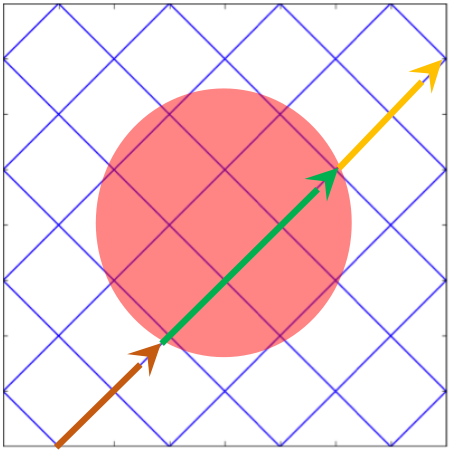
\includegraphics[width=\linewidth]{figures/laydown/kord_tracks_2D.png}
		\caption{}
		\label{fig:sample-tracks-a}
	\end{subfigure}
	\begin{subfigure}[b]{0.35\textwidth}
		\centering
		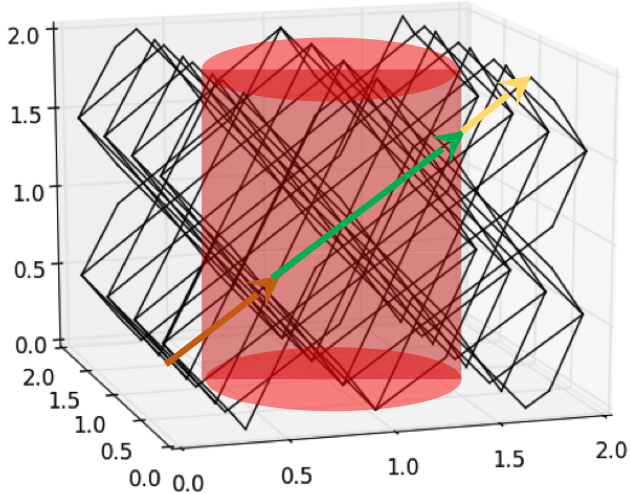
\includegraphics[width=\linewidth]{figures/laydown/kord_tracks_3D.png}
		\caption{}
		\label{fig:sample-tracks-b}
	\end{subfigure}
	\caption[]{Illustration of (a) 2D and (b) 3D cyclic tracks for a pin-cell geometry.}
	\label{fig:sample-tracks}
\end{figure}


There are a variety of ways cyclic tracking can be enforced by adjusting MOC ray parameters. Depending on the track laydown algorithm, the parameter adjustment can be significant, often inserting far more tracks than necessary. Inefficient track laydown algorithms can lead to an order of magnitude increase in the number of tracks required for realistic PWR problems~\cite{shaner-laydown}. Since the computational cost of MOC scales directly with the number of tracks, an order of magnitude increase in the number of tracks translates directly into an order of magnitude increase in the run time. \textbf{This thesis implements track laydown using Modular Ray Tracing (MRT), which has quite flexible constraints with a minimal number of additional track insertions}~\cite{liu_mrt}.


%%%%%%%%%%%%%%%%%%%%
\subsection*{On-the-fly Ray Tracing}

After tracks are laid across the geometry, each track is subdivided into segments at each spatial region boundary using a ray tracing algorithm. MOC equations are solved for each segment. The algorithm used to retrieve ray tracing information can have a significant impact on computational performance. Traditional MOC implementations conduct ray tracing upfront, storing the associated ray tracing data, and referencing it during the solve. While this approach is straightforward, its memory and compute requirements for 3D MOC are prohibitive, even for small problems, due to the vast number of segments present in 3D MOC simulations. The explicit storage of 3D segments in OpenMOC for a single assembly of the C5G7 benchmark with coarse MOC parameters required 79 GB~\cite{physor2016otf}. Reducing the memory footprint is important for improving computational efficiency.

In this thesis, \textbf{an alternative approach is presented that greatly reduces the segment storage by taking advantage of the extruded geometry structure common to many reactor physics problems}. This approach saves no 3D segment data, but instead stores 2D radial ray tracing information and combines this information with 1D axial meshes to compute 3D intersections on-the-fly~\cite{physor2016otf}.

Two on-the-fly ray tracing approaches are introduced in this thesis. One approach ray traces each 3D track individually. Another ray traces an entire grouping of tracks together which have the same direction with polar angle $\theta$, stacked in the axial direction and separated by constant spacing $\delta z$. The group of tracks, referred to as a $z$-stack, allows for analytic calculation of the first and last track indexes within the stack that intersect each region. This ray tracing process is depicted in Figure~\ref{fig::stack_tracing}. Both ray tracing approaches offer significant memory reduction with minimal computational overhead.

\begin{figure}[ht!]
	\centering
	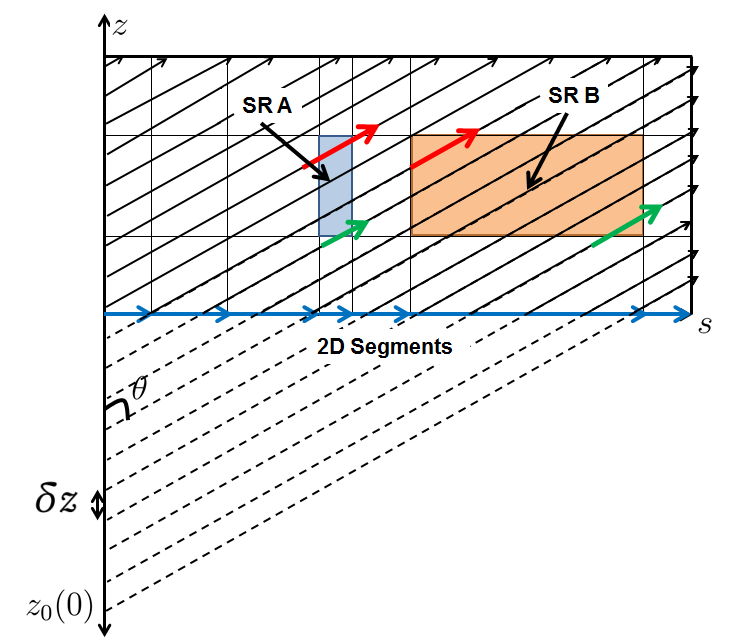
\includegraphics[width=0.75\linewidth]{figures/ph2016/stack_tracing.png}
	\caption{Illustration of the on-the-fly axial ray tracing process for an entire $z$-stack where the lowest track intersects the $z$-axis at $z_0(0)$. In Source Region (SR) A, multiple tracks traverse the entire 2D segment length. In SR B, no tracks traverse the entire 2D segment length.}
	\label{fig::stack_tracing}
\end{figure}


\newpage
%%%%%%%%%%%%%%%%%%%%
\subsection*{Linear Source Approximation}

A flat source approximation is typically used in MOC implementations whereby the spatial shape of the total source in each mesh cell is approximated by a constant. While this approximation is convenient and used by many~\cite{kochunas, liu_mrt, dragon_3d_moc, apollo3_vv, cactus_3d, mockingbird}, a linear approximation can potentially reduce the computational requirements of simulating a fully converged reactor physics problem. The linear source approximation increases the computational cost for a fixed discretization but the higher order source can capture source gradients, allowing for a much coarser spatial mesh discretization while maintaining solution accuracy~\cite{ferrer2012linear}. In this thesis, \textbf{the track-based linear source approximation introduced by Ferrer}~\cite{ferrer2015linear} \textbf{for 2D MOC is extended to 3D MOC} and implemented in OpenMOC.


%FIXME: Ben wants a picutre, explanation of discretization

To evaluate on-node performance, the Single Domain Single Assembly (SDSA) test problem is created which is a nearly cubic cutout of the BEAVRS reactor. Specifically, the test problem represents a single assembly radially that has been extruded 20 cm in height with reflective boundaries on all bounding surfaces. It is meshed with the discretization expected to accurately simulate the full core. Cross-sections are formed for each unique material in 70 energy groups. The size of the cutout was chosen to be the largest cutout to reasonably fit on one node of the Argonne BlueGene/Q supercomputer which has a memory limit of 16 GB per node.

Singe-thread performance is often useful for determining the efficiency of an MOC implementation. One useful performance metric is ``integration time'' which refers to the time required to compute the angular flux variation over one segment and tally its contribution to the local scalar flux for one energy group. Since the number of segments increases with the size of the problem, integration time is less problem-dependent than other performance metrics such as run-time. Single thread computational results of both on-the-fly ray tracing schemes are presented in Table~\ref{tab:rt-single-thread} for the SDSA test problem with fixed mesh.

\begin{table}[ht]
	\centering
	\caption{Single thread performance of OpenMOC using one node of the Falcon supercomputer}
	\medskip
	\begin{tabular}{l|l|l}
		\hline
		Ray Tracing Scheme & Source Approximation & Integration Time (ns) \\
		\hline
		By Track  & Flat & 12.2 +/- 0.01 \\
		By $z$-Stack & Flat & 10.8 +/- 0.01 \\
		\hline
		By Track  & Linear & 31.41 +/- 0.08 \\
		By $z$-Stack & Linear & 29.87 +/- 0.03 \\
		\hline
	\end{tabular}
	\label{tab:rt-single-thread}
\end{table}

Both ray tracing methods are able to achieve $\approx 10$ ns integration time with the flat source approximation. The linear source approximation adds a factor of two to three overhead. However, the higher-order source approximation allows the spatial mesh to be significantly coarsened while maintaining solution accuracy. For both flat and linear source solvers, on-the-fly ray tracing by $z$-stack slightly outperforms on-the-fly ray tracing by individual 3D track. 

OpenMOC uses OpenMP shared memory parallelism~\cite{openmp} on each node. The scaling results of the linear source solver with ray tracing by $z$-stack are shown in Figure~\ref{fig:rt-parallel-ls-cetus} using the Cetus partition of the Argonne BlueGene/Q supercomputer to solve the SDSA test problem. This machine has 16 cores per node and hyper-threads allow for improved resource utilization with up to 64 threads. It is important to note that beyond 16 threads, ideal speedup is not expected as threads must share the computation resources of the 16 cores. At 16 threads, the achieved speedup is 90.9\% of ideal.

\begin{figure}[ht!]
	\centering
	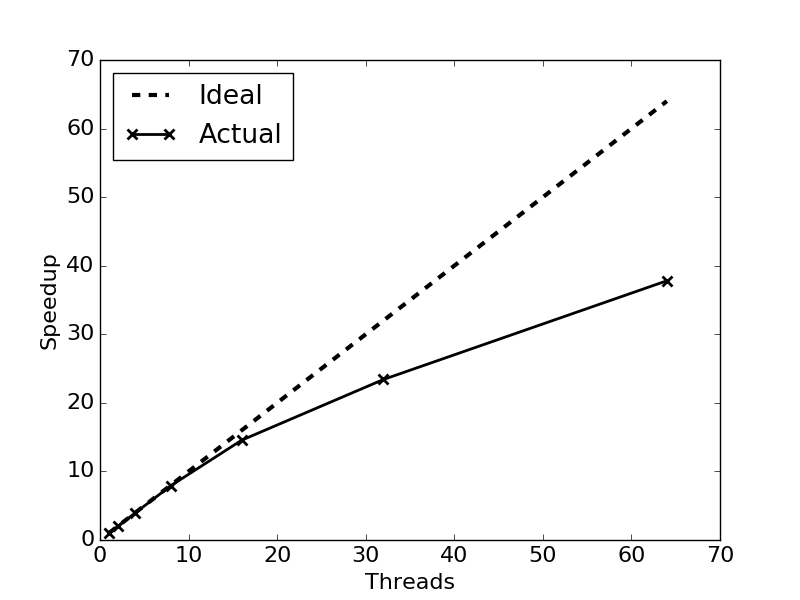
\includegraphics[width=0.75\linewidth]{figures/results/performance/ls-parallel-scaling-stacks-cetus.png}
	\caption{Strong scaling performance of the linear source solver on the SDSA test problem using the Cetus partition of the Argonne BlueGene/Q supercomputer with on-the-fly ray tracing by $z$-stacks.}
	\label{fig:rt-parallel-ls-cetus}
\end{figure}


%%%%%%%%%%%%%%%%%%%%
\subsection*{Domain Decomposition}

Solvers need to be able to scale to many computational nodes in order to solve large reactor physics problems, such as the BEAVRS benchmark. While shared memory parallelism is feasible for on-node scaling, it is infeasible for inter-node scaling due to significant latency when transferring information between nodes. Therefore, \textbf{a hybrid parallelism model is adopted in which on-node scaling is handled with OpenMP shared memory parallelism and inter-node scaling is handled with spatial domain decomposition using MPI}~\cite{mpi}.

Scalable spatial domain decomposition was implemented in OpenMOC by partitioning the geometry using a uniform Cartesian grid into many geometrical sub-domains. Each sub-domain represents an encapsulated MOC problem, only relying on other sub-domains for boundary angular fluxes and a few global variables such as normalization factors and the eigenvalue. To communicate angular flux information, the same modular track laydown is used on each sub-domain in which tracks naturally link at boundaries. By having a modular track laydown~\cite{liu_mrt}, each sub-domain can easily connect track indexes with periodic track indexes.

In addition to communicating MOC information, the same spatial domain decomposition is also applied to the CMFD acceleration. The CMFD equations are iteratively solved using a red/black SOR scheme in which ghost cell scalar fluxes are communicated on each iteration.

Numerous scaling studies were conducted to ensure efficient parallel scaling of the domain decomposition implementation to many nodes. One such study replicated the SDSA test problem in a cubic 3D lattice. Weak scaling tests, in which problem size per node is kept constant, were conducted on the Cetus partition of the Argonne BlueGene/Q supercomputer with each node assigned one of the lattice cells (equivalent to one SDSA geometry). The results are presented in Figure~\ref{fig:dd-ws-3D-eff}, showing greater than 90\% parallel efficiency for all configurations. The largest case involves a $12 \times 12 \times 12$ lattice consuming 1728 nodes (27,648 cores), resulting in an efficiency of 92\%.
	
\begin{figure}[h!]
	\centering
	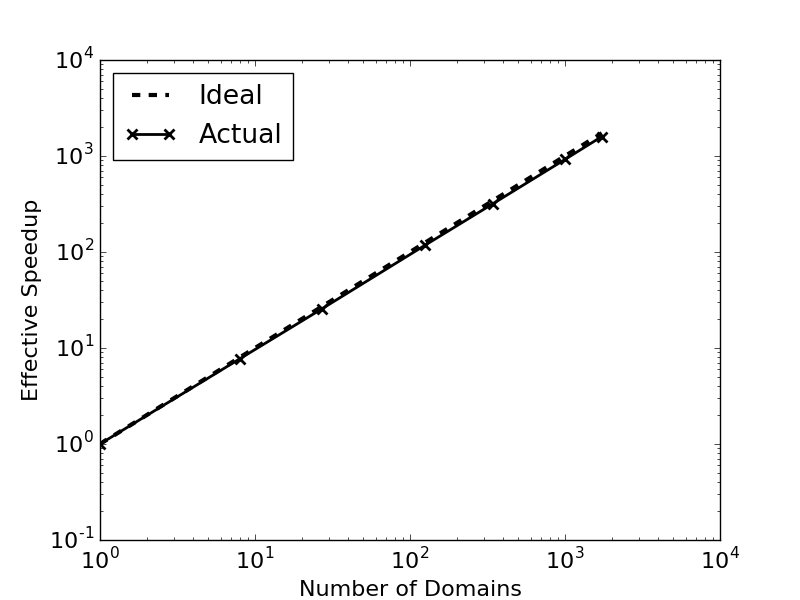
\includegraphics[width=0.75\linewidth]{figures/DD/dd-ws-3D-eff.png}
	\caption[]{Weak scaling of the domain decomposition implementation of the linear source solver on a replicated 3D lattice of the SDSA test problem.}
	\label{fig:dd-ws-3D-eff}
\end{figure}

%%%%%%%%%%%%%%%%%%%%%%%%%%%%%%%%%%%%%%%%%%%%%%%%%%%%%%%%%%%%%%%%%%%%%%%%%%%%%%%%
\section*{Convergence of Source Iteration}

The OpenMOC solver described in this thesis relies on source iteration used in conjunction with CMFD acceleration to solve the MOC equations. While convergence of source iteration is straightforward for any set of physical cross-sections, the use of transport-corrected cross-sections can cause convergence issues. Transport correction is required to produce accurate solutions using OpenMOC when using the isotropic source assumption.

\textbf{This thesis introduces a novel strategy to overcome the convergence issues of source iteration using damping of the MOC scalar fluxes, termed diagonal stabilization}. A robust description of the source of convergence issues with transport-corrected cross-sections is discussed in this thesis. Specifically, the diagonal stabilization method damps the update of MOC fluxes $\phi_{\mathbf{n}}$ in iteration $\mathbf{n}$ as
\begin{equation}
\nonumber
\phi_{\mathbf{n}+1} = \beta \phi_{\mathbf{n}+1/2} + (1-\beta) \phi_{\mathbf{n}} 
\end{equation}
where iteration $\mathbf{n}+1/2$ refers to the computed solution without damping. The damping coefficient $\beta$ is chosen based on the ratio of within-group scattering to transport cross-section for each region and energy group.

Diagonal stabilization is tested on multiple reactor physics problems, including the full core BEAVRS model with in-scatter transport correction, showing that it is necessary to achieve convergence using a reduced CMFD group structure. A comparison of the convergence behavior with and without diagonal stabilization is shown in Figure~\ref{fig:fc-3D-ls} for the BEAVRS full core model using the OpenMOC linear source solver with coarse MOC ray parameters, showing an inability to converge the problem without diagonal stabilization.
	
\begin{figure}[ht!]
	\centering
	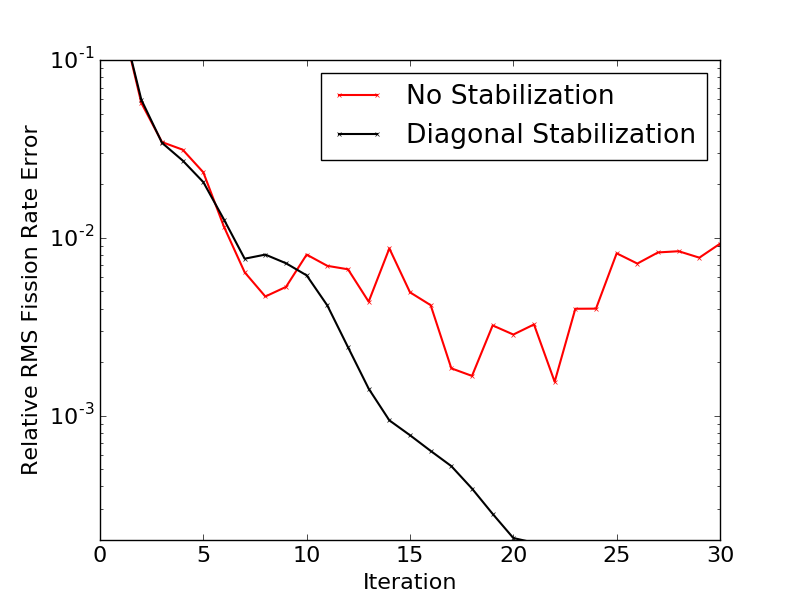
\includegraphics[width=0.65\linewidth]{figures/convergence/full-core-3D-ls.png}
	\caption{Convergence behavior of OpenMOC's linear source solver on the full core BEAVRS benchmark with and without Diagonal Stabilization.}
	\label{fig:fc-3D-ls}
\end{figure}

It is important to note that this stabilization strategy has implications for all neutron transport solvers -- not just MOC solvers. Any solver which relies on source iteration has the potential to experience these same convergence issues when using transport-corrected cross-sections. Due to its wide-ranging applicability, this diagonal stabilization method is one of the most important contributions of this thesis to the reactor physics community. 


%%%%%%%%%%%%%%%%%%%%%%%%%%%
\section*{Simulation Results}

%%%%%%%%%%%%%%%%%%%%%%%%%%%%%%%%%%%%%%%%%%%%%%%%%
\subsection*{Single Assembly Sensitivity Studies}

After the OpenMOC solver was fully implemented, sensitivity to the MOC parameters was tested. All results in this thesis use a 70 group cross-section library formed from OpenMC Monte Carlo simulations of the BEAVRS benchmark using the \texttt{mgxs} package~\cite{boyd2017thesis}. \text{In-scatter} transport correction was applied to all cross-sections. A variety of cutouts from the BEAVRS model were selected to test the sensitivity to MOC ray and mesh parameters. The models include a 2D extruded BEAVRS core in which a thin axial region is simulated with axially reflective boundary conditions and a single assembly with full axial detail. The single assembly is used for the majority of sensitivity tests, particularly for the sensitivities to 3D parameters. Converged radial and axial fission distributions are presented in Figure~\ref{fig:single-assembly-dist} for the single assembly model.


\begin{figure}[h!]
	\centering
	\begin{subfigure}[b]{0.45\textwidth}
		\centering
		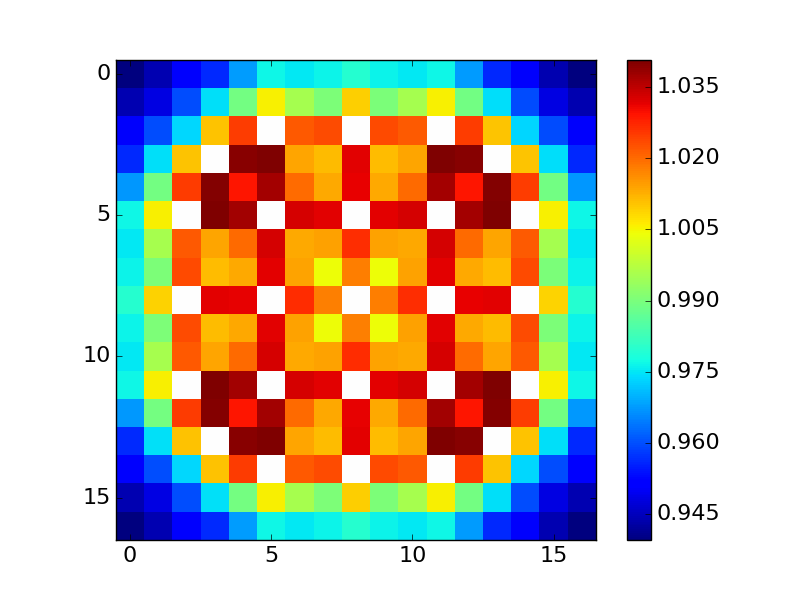
\includegraphics[width=\linewidth]{figures/results/rr-plots/single-assembly-radial.png}
		\caption{}
		\label{fig:single-assembly-radial}
	\end{subfigure}
	\begin{subfigure}[b]{0.45\textwidth}
		\centering
		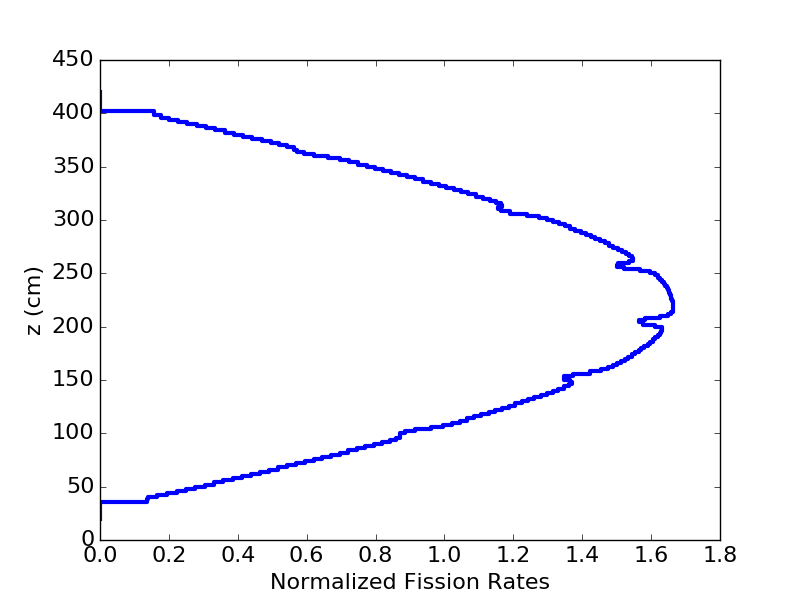
\includegraphics[width=\linewidth]{figures/results/rr-plots/single-assembly-axial.png}
		\caption{}
		\label{fig:single-assembly-axial}
	\end{subfigure}
	\caption[]{The radial (a) and axial (b) fission rate distribution of the single assembly model.}
	\label{fig:single-assembly-dist}
\end{figure}

While radial MOC parameters have been previously studied in great detail for 2D MOC solvers~\cite{rhodes2006casmo}, the 3D MOC parameters have not been thoroughly examined. Parameter convergence is determined by comparing computed results with a fine parameter reference solution. An accuracy criteria of less than 1.0\% Root Mean Square (RMS) and 3.0\% maximum pellet-wise fission rate error is used to determine the appropriate parameters where each pellet-wise fission rate is defined by the fission rate within a 2.0 cm zone of a fuel rod. An eigenvalue bias of less than 20 pcm is also required. The resulting MOC parameters are shown in Table~\ref{tab:final-params}. A depiction of the required radial mesh chosen for a single assembly is presented in Figure~\ref{fig:assembly-mesh}.

\begin{table}[ht]
	\centering
	\caption{MOC ray and mesh parameters determined to accurately and efficiently simulate typical PWR problems}
	\medskip
	\begin{tabular}{lc}
		\hline
		Radial Ray Spacing & 0.05 cm \\
		Axial Ray Spacing & 0.75 cm \\
		Number of Azimuthal Angles & 64 \\
		Number of Polar Angles & 10 \\
		\hline
		Number of Fuel Sectors & 4 \\
		Number of Guide Tube Sectors & 8 \\
		Number of Moderator Sectors & 8 \\
		Axial Source Height & 2.0 cm \\
		Radial Reflector Mesh & $3\times 3$ cells per pin-cell mesh \\
		\hline
		CMFD Cell Height & 2.0 cm \\
		Number of CMFD Energy Groups & 8 \\
		\hline
	\end{tabular}
	\label{tab:final-params}
\end{table}
		
\begin{figure}[ht!]
	\centering
	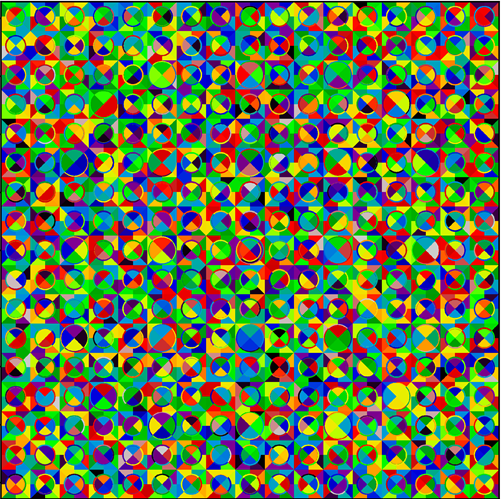
\includegraphics[width=0.7\linewidth]{figures/moc_mesh.PNG}
	\caption{Radial mesh discretization of a single assembly}
	\label{fig:assembly-mesh}
\end{figure}

\newpage
%%%%%%%%%%%%%%%%%%%%%%%%%%%%%%%%%%%%%%%%%%%%%%%%%
\subsection*{Full Core Results}


Using the MOC parameters presented in Table~\ref{tab:final-params}, the BEAVRS benchmark is simulated on the Mira partition of the Argonne BlueGene/Q supercomputer using the linear source 3D MOC solver in OpenMOC. The resulting radially and axially integrated reaction rates are presented in Figure~\ref{fig:full-core-radial} and Figure~\ref{fig:full-core-axial}.

\begin{figure}[ht!]
	\centering
	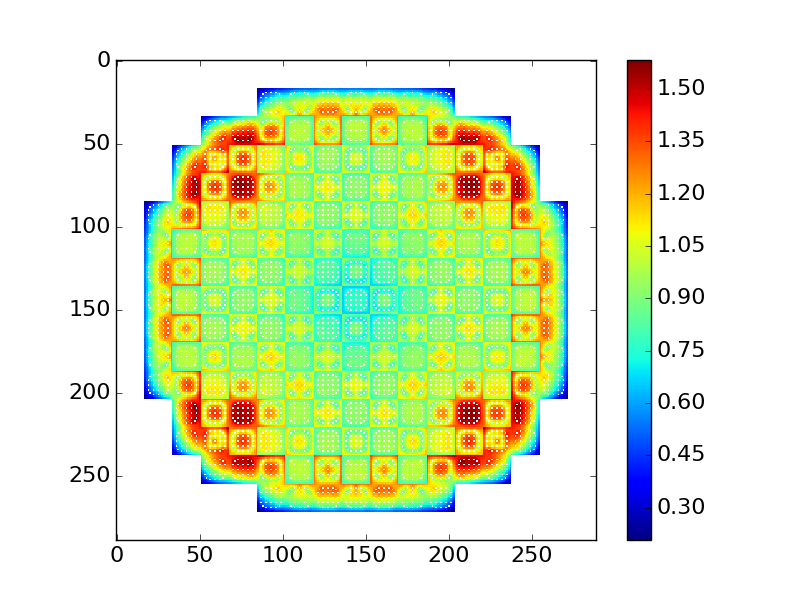
\includegraphics[width=0.65\linewidth]{figures/results/rr-plots/beavrs-3d-radial.png}
	\caption{Radial fission rate distribution for the BEAVRS benchmark formed by OpenMOC with reaction rates axially integrated.}
	\label{fig:full-core-radial}
\end{figure}

\begin{figure}[ht!]
	\centering
	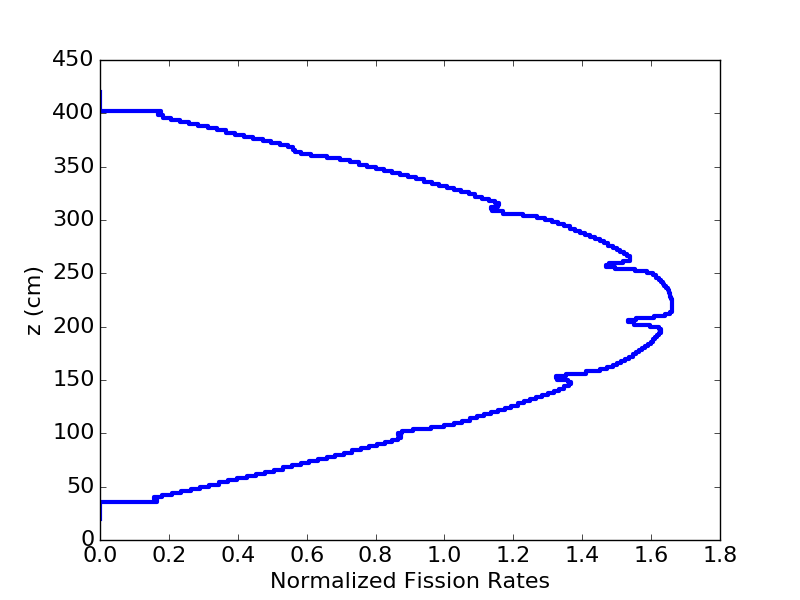
\includegraphics[width=0.65\linewidth]{figures/results/rr-plots/beavrs-3d-axial.png}
	\caption{Axial fission rate distribution for the BEAVRS benchmark formed by OpenMOC with reaction rates radially integrated.}
	\label{fig:full-core-axial}
\end{figure}

\newpage
The OpenMOC results are compared with an OpenMC Monte Carlo solution from which the cross-sections were derived. The Monte Carlo simulation used 400 batches (300 inactive, 100 active) with $2 \times 10^8$ particles per batch. A comparison of the OpenMOC and OpenMC solutions is presented in Table~\ref{tab:openmc-comparison} in which fission rates are calculated on a pellet-wise scale (2.0 cm axial height).

\begin{table}[ht]
	\centering
	\caption{Simulation accuracy of OpenMOC relative to an OpenMC reference solution}
	\medskip
	\begin{tabular}{l|l|c|c}
		%\hline
		&                               & Avg. Fission Rate & RMS Fission \\
		& $k_{\textit{eff}}$ eigenvalue & Std. Dev.         & Rate Error \\
		\hline
		OpenMC  & 0.99927 +/- 0.00001  & 1.82\% & --     \\
		OpenMOC & 0.99677                         & --     & 2.14\% \\
		\hline
	\end{tabular}
	\label{tab:openmc-comparison}
\end{table}


Notice that since Monte Carlo simulations introduce statistical noise, each pellet-wise Monte Carlo fission rate has an associated standard deviation. The RMS pellet-wise fission rate error of OpenMOC is 2.14\% which is close to the average standard deviation of OpenMC tallies. The radial and axial error distributions are presented in Figure~\ref{fig:openmc-comp-rad} and Figure~\ref{fig:openmc-comp-ax}, respectively, showing a radial tilt across the core.


\begin{figure}[ht!]
	\centering
	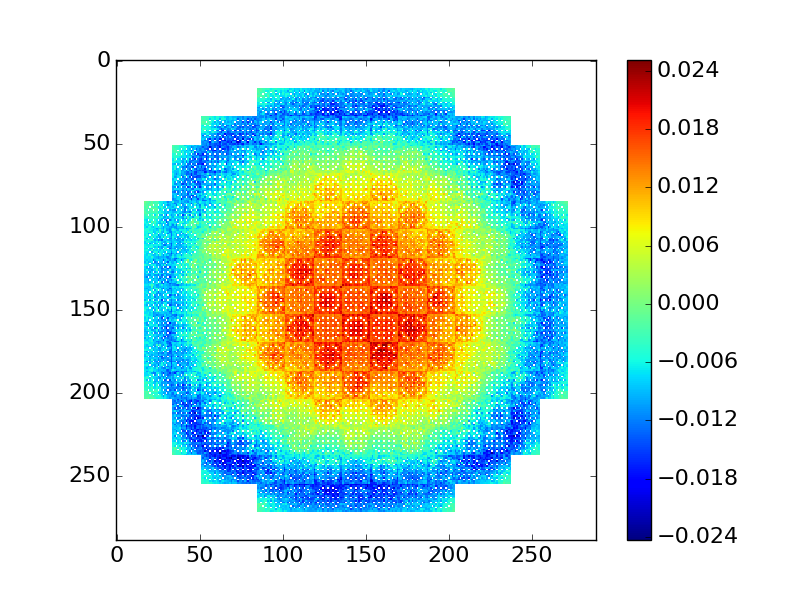
\includegraphics[width=0.8\linewidth]{figures/results/full-core/radial_diff_v_openmc.png}
	\caption{Radial distribution of normalized fission rate errors of OpenMOC compared with a reference OpenMC solution on the BEAVRS benchmark.}
	\label{fig:openmc-comp-rad}
\end{figure}

\begin{figure}[ht!]
	\centering
	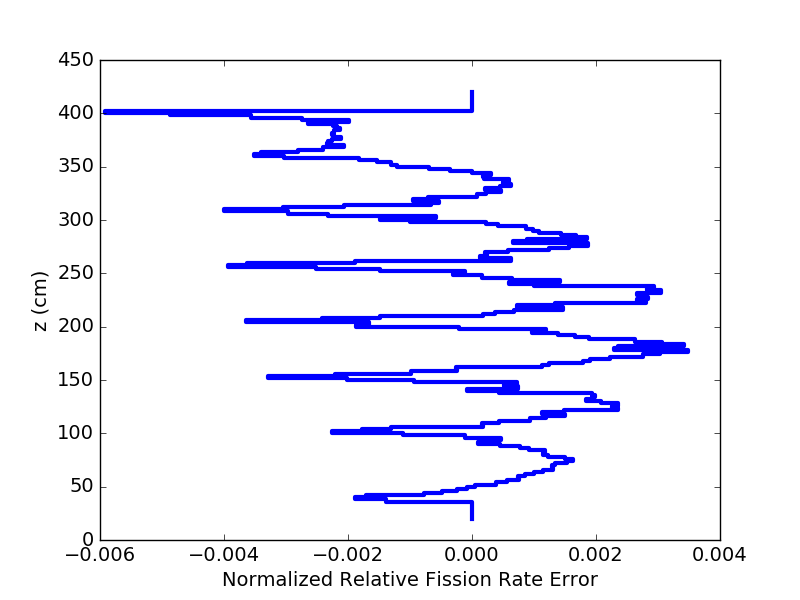
\includegraphics[width=0.8\linewidth]{figures/results/full-core/axial_diff_v_openmc.png}
	\caption{Axial distribution of normalized fission rate errors of OpenMOC compared with a reference OpenMC solution on the BEAVRS benchmark.}
	\label{fig:openmc-comp-ax}
\end{figure}


To ensure the gross fission rate distribution is simulated with reasonable accuracy, assembly-integrated fission rates are compared. Figure~\ref{fig:assembly-rr} shows these assembly rate errors and the associated OpenMC reference folded into a 1/8 map. Similar to the radial distribution shown in Figure~\ref{fig:openmc-comp-rad}, the error again appears as a pure tilt across the core. This tilt is due to the particular transport correction that is not able to fully capture the effects of anisotropic scattering. It is possible that a better transport correction -- particularly in reflector regions -- would be able to eliminate this tilt. However, accurate cross-section formation is not the objective of this thesis and other ongoing projects at MIT are seeking to improve the transport correction.

\begin{figure}[ht!]
	\centering
	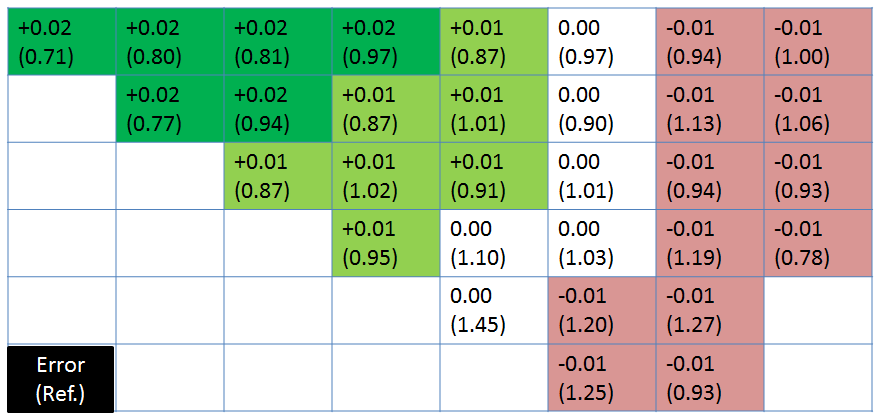
\includegraphics[width=\linewidth]{figures/results/full-core/folded-1-8-core-assembly-rr.png}
	\caption{1/8 core folded assembly fission rate error of OpenMOC compared with the reference OpenMC solution for the BEAVRS benchmark.}
	\label{fig:assembly-rr}
\end{figure}

The computational requirements of the full core solution in OpenMOC is presented in Table~\ref{tab:full-core-comp-req}. Note that while the number of core-hours required to converge the problem is high (717,465), the solution was computed on the Argonne BlueGene/Q supercomputer, which has extremely slow cores for energy efficiency reasons. The requirements on modern computing cores, such as those on the Falcon supercomputer, is estimated by comparing the integration time per core of the SDSA problem on the Falcon supercomputer (48.96 ns/core) to those on the Argonne BlueGene/Q supercomputer (175.36 ns/core) for one node using all available cores. However, this case cannot be explicitly simulated on Falcon due to the small aggregate memory of the Falcon supercomputer.

\begin{table}[ht]
	\centering
	\caption{Computational requirements of OpenMOC on the full core 3D BEAVRS benchmark using the Mira partition of the Argonne BlueGene/Q supercomputer}
	\medskip
	\begin{tabular}{l|l}
		\hline
		Runtime & 7.76 hours \\
		Number of Transport Sweeps & 20 \\
		Nodes & 5780 ($17 \times 17 \times 20$) \\
		CPU Cores & 92480 \\
		Integration Time per Core & 256.7 ns / core \\
		Computational Cost & 717,465 core-hours \\
		Estimated Computational Cost on Falcon & $\approx$ 200,314 core-hours \\
		\hline
	\end{tabular}
	\label{tab:full-core-comp-req}
\end{table}

Further analysis of the computational profile is presented in Table~\ref{tab:full-core-comp-prof}. The results show the computational overhead of CMFD acceleration was insignificant. In addition, the time spent communicating boundary angular fluxes between domains was quite small. However, there was significant idle time between sweeps when nodes are waiting for other nodes to finish their current transport sweeps. This is an indication of load imbalance due to more work being required in core regions than in reflector regions.

\begin{table}[ht]
	\centering
	\caption{Computational profile of OpenMOC on the full core 3D BEAVRS benchmark using the Mira partition of the Argonne BlueGene/Q supercomputer}
	\medskip
	\begin{tabular}{lll|c|c}
		\hline
		& & & Computation & Fraction of \\
		\multicolumn{3}{c|}{Solver Component} & Time (s) & Runtime\\
		\hline
		Total & & & $2.79 \times 10^4$ & 100\% \\
		& Transport Sweeps & & $2.67 \times 10^4$ & 95.8\% \\
		& & Angular Flux Communication & $7.05 \times 10^2$ & 2.5\% \\
		& & Idle Time Between Sweeps & $7.74 \times 10^3$ & 27.7\% \\
		& CMFD Solver & & $97.4$ & 0.3\% \\		
		\hline
	\end{tabular}
	\label{tab:full-core-comp-prof}
\end{table}

\newpage

            
In order to verify that the chosen MOC parameters where sufficient in accurately converging the solution, simulations are conducted in which each 3D parameter is refined, with the results shown in Table~\ref{tab:fc-param-sensitivity}. Ideally, all parameters should be refined together, but the computational burden would be too large to run on Mira. Therefore, each parameter is refined separately. Due to memory constraints, ray parameters were only able to be refined by $\approx 1.5 \times$ but the axial mesh could be refined by a factor of 2. These results indicate that the solution nearly satisfies to the desired criteria of less than 1.0\% pellet-wise RMS fission rate error, less than 3.0\% maximum error, and less than 20 pcm bias with respect to finer parameter solutions. In order to strictly adhere to the criteria, the axial mesh would need to be slightly refined.

\begin{table}[ht]
	\centering
	\caption{Differences observed from refining 3D MOC parameters for the BEAVRS benchmark relative to the first solution}
	\medskip
	\begin{tabular}{l|l|l|c|c|c}
		\hline
		Polar  & Axial Ray & Source & $k_{\textit{eff}}$  & RMS Fission & Max Fission \\
		Angles & Spacing   & Height & Bias                & Rate Diff. & Rate Diff. \\
		\hline
		10 & 0.75 cm & 2.0 cm & --     & --     & --  \\
		14 & 0.75 cm & 2.0 cm & 2 pcm  & 0.51\% & 1.92\%  \\
		10 & 0.50 cm & 2.0 cm & 5 pcm  & 0.41\% & 1.76\%  \\
		10 & 0.75 cm & 1.0 cm & 13 pcm & 0.28\% & 3.33\%  \\
		\hline
	\end{tabular}
	\label{tab:fc-param-sensitivity}
\end{table}


\clearpage

%%%%%%%%%%%%%%%%%%%%%%%%%%%%%%%%%%%%%%%%%%%%%%%%%%%%%%%%%%%%%%%%%%%%%%%%%%%%%%%%
\section*{Conclusions}

The main goal of this thesis was to develop a 3D MOC solver capable of accurately and efficiently simulating LWR models for a fixed but reasonable choice of cross-sections. This goal was motivated by the desire to develop methods which can explicitly handle axial as well as radial variation within PWR reactor cores. The following summarizes the key accomplishments demonstrated by this thesis to meet this challenge:

\begin{itemize}

\item \textbf{The implementation of an efficient 3D MOC solver.} A 3D MOC solver was implemented in OpenMOC which is capable of efficiently solving the MOC equations using an efficient track laydown, on-the-fly ray tracing, and spatial domain decomposition. In addition, an efficient linear source solver was added, allowing for accurate solutions with relatively coarse mesh.

\item \textbf{Theoretical and practical evaluation of source iteration convergence.} The convergence of transport codes using source iteration (such as MOC) with transport-corrected cross-sections has plagued researchers in the past. In this thesis, a robust theoretical framework is introduced to understand convergence characteristics. The diagonal stabilization scheme was presented which alleviates the convergence issues.

\item \textbf{3D MOC parameter refinement studies.} Since previous 3D MOC solvers have not been capable of solving large PWR problems, parameter refinement studies have not been fully explored. In this thesis, the sensitivity of solution accuracy to each 3D MOC parameter is thoroughly explored.

\item \textbf{Evaluation of computational requirements for solving full core PWR problems.} Since OpenMOC is the first solver capable of solving the BEAVRS benchmark with deterministic methods, it provides a useful indicator for the computational cost of solving such a large problem.

\end{itemize}

Past 3D deterministic solvers have not been capable of fully resolving full core PWR models to pellet-level precision. This thesis shows that these large scale simulations are now possible with careful consideration of implementation details critical to performance. These simulations can provide useful insight into the neutron behavior of rector geometries with complex geometric detail, such as the Westinghouse AP 1000\texttrademark. With this insight, safety margins could potentially be lowered, leading to more efficient and economic operation of modern nuclear reactors.

%FIXME: Perspectives on Future Solvers ???

%%%%%%%%%%%%%%%%%%%%%%%%%%%%%%%%%%%%%%%%%%%%%%%%%%%%%%%%%%%%%%%%%%%%%%%%%%%%%%%%
%%%%%%%%%%%%%%%%%%%%%%%%%%%%%%%%%%%%%%%%%%%%%%%%%%%%%%%%%%%%%%%%%%%%%%%%%%%%%%%%
% BIBLIOGRAPHY

\begin{singlespace}
\bibliographystyle{ans}
\bibliography{references}
\end{singlespace}

\end{document}
